\chapter{Systemarchitektur}

\section{Architekturüberblick}
Gesamtsicht auf die Architektur der Lösung (Backend, Frontend, Datenbank).

\begin{figure}[!h]
    \centering
    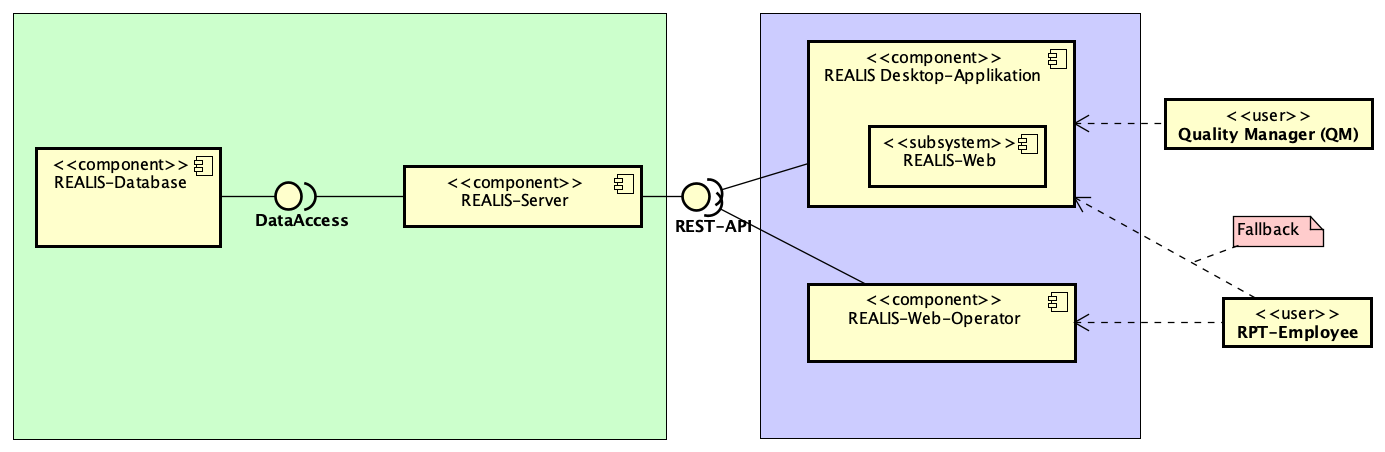
\includegraphics[width=1\textwidth]{bilder/REALIS-Komponentendiagramm.png}
    \caption{REALIS Komponentendiagramm}
    \label{fig:realis-komponentendiagramm}
\end{figure}

\section{Datenbankdesign}
Struktur der Oracle-Datenbank, wichtige Tabellen und Beziehungen.

\begin{figure}[!h]
    \centering
    \makebox[\textwidth]{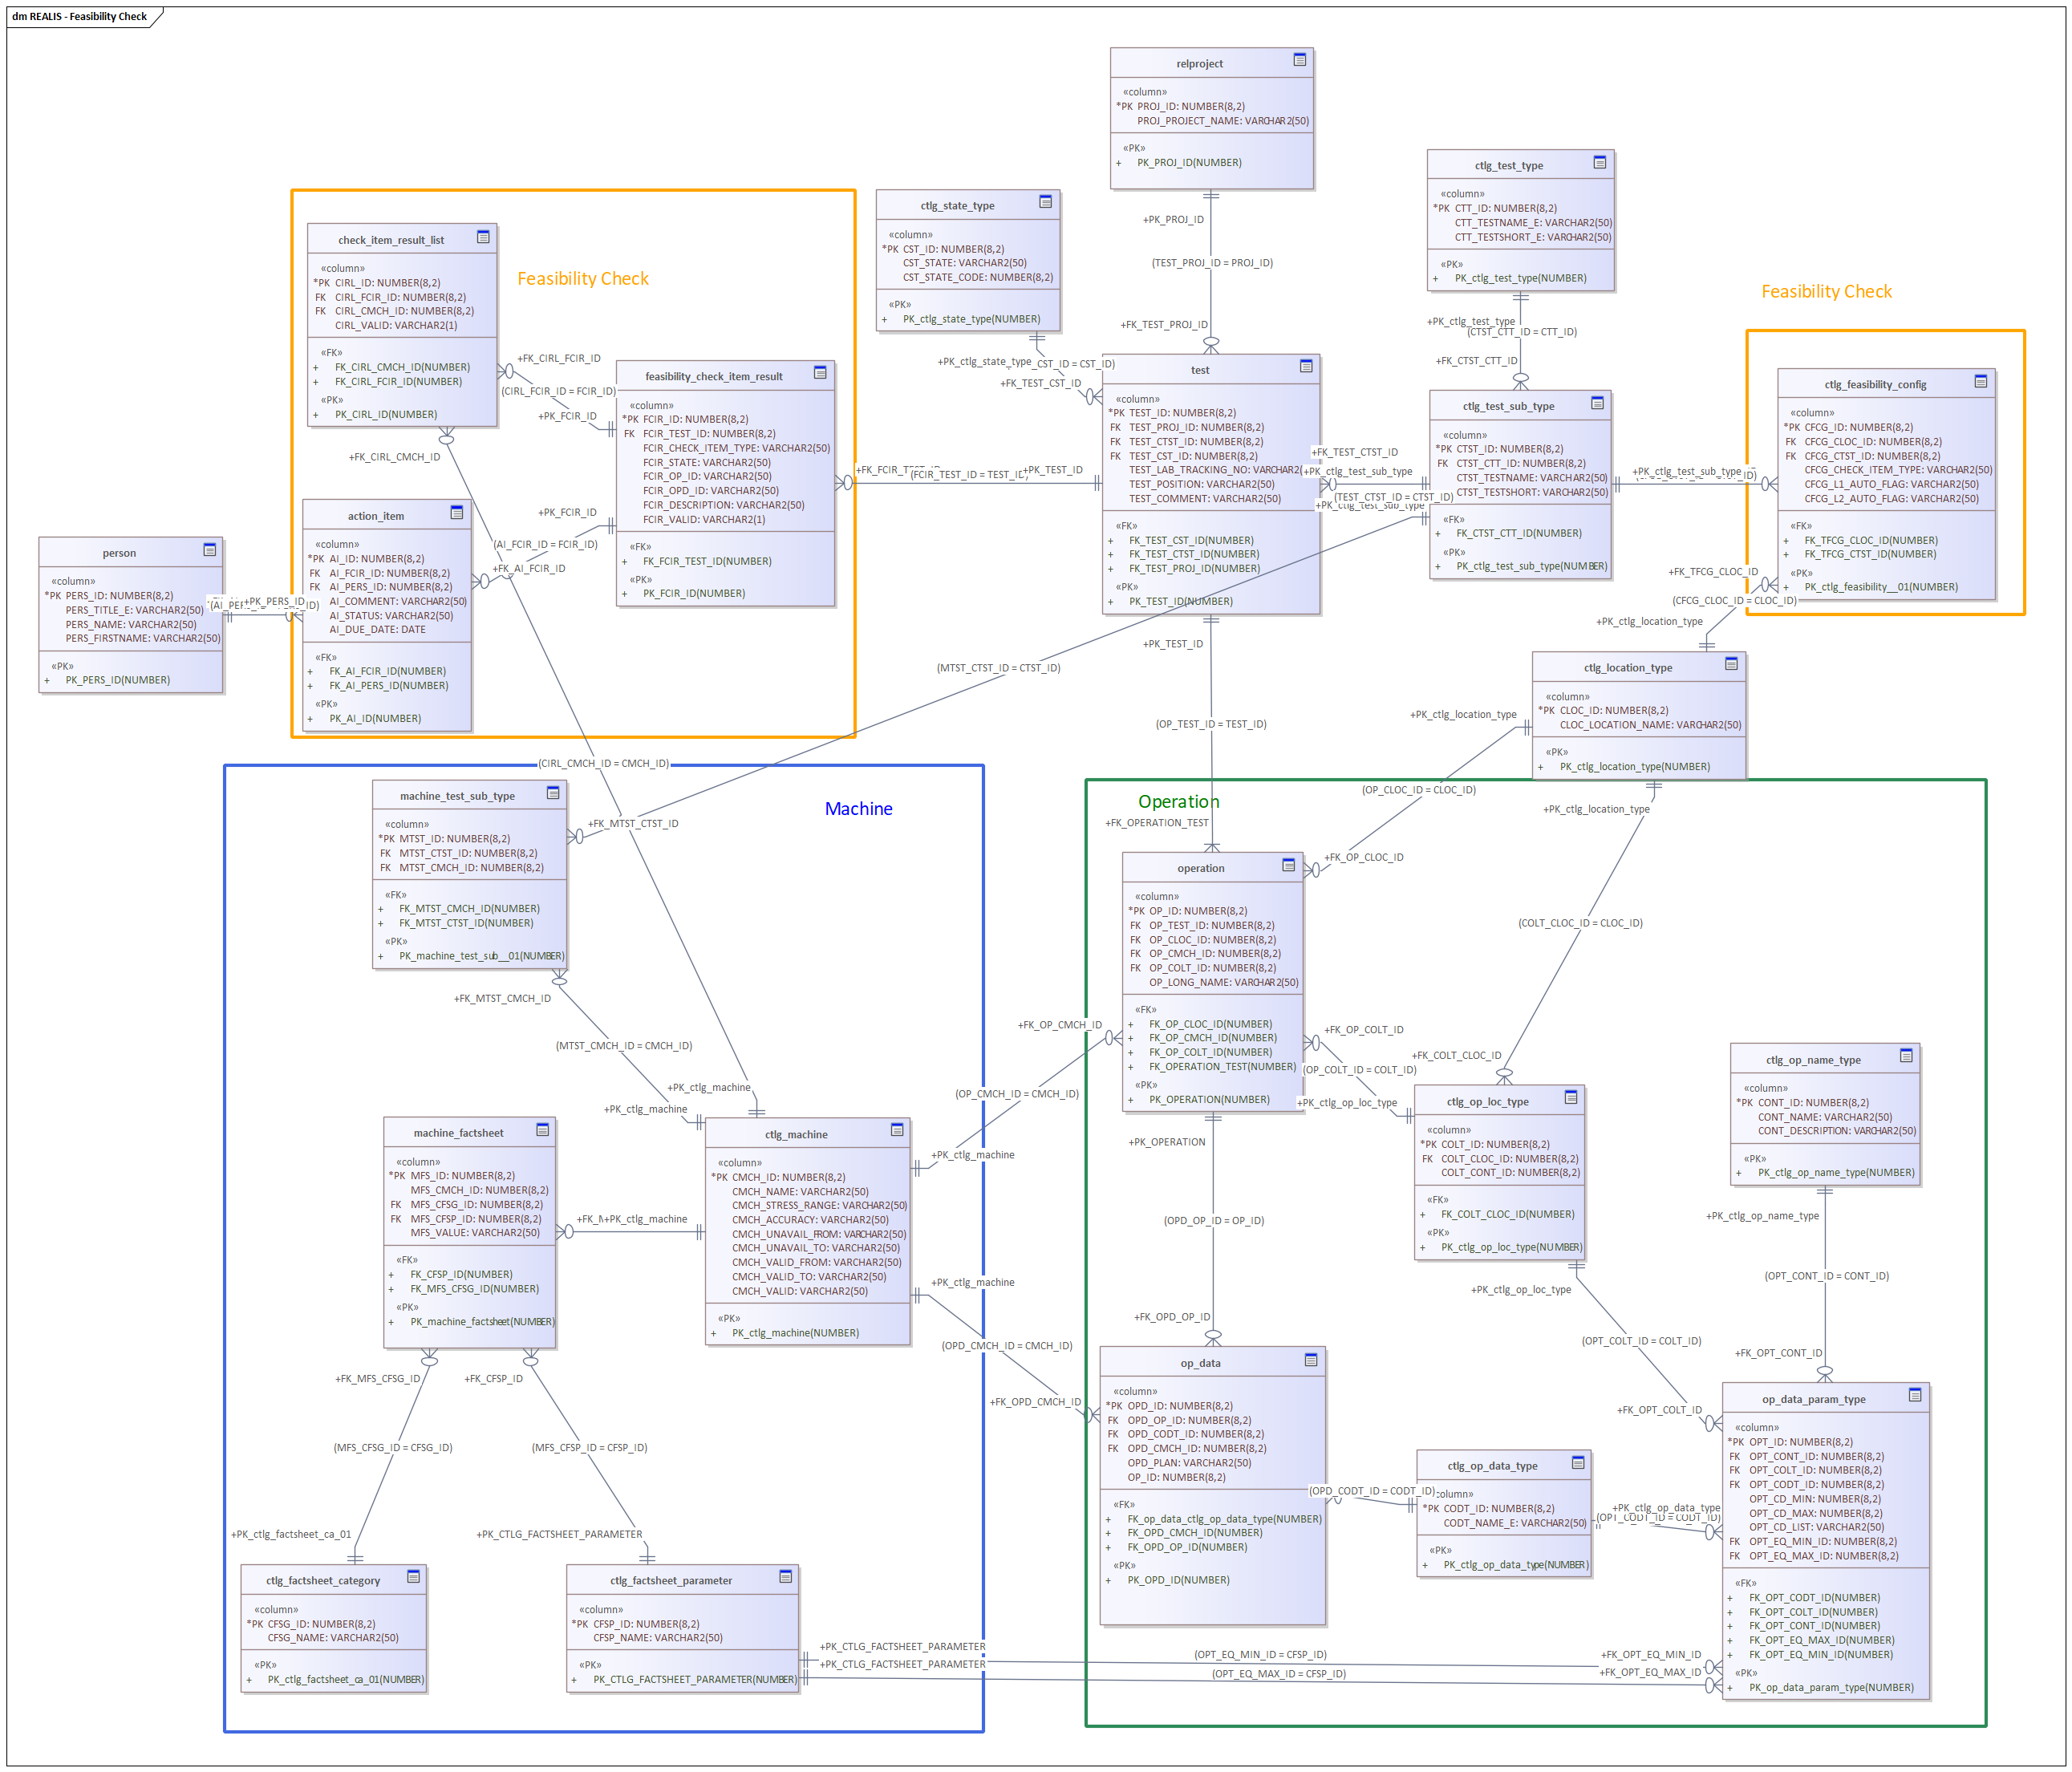
\includegraphics[width=0.98\paperwidth]{bilder/REALIS-Datenbankmodell.png}}
    \caption{REALIS Datenbankdesign}
    \label{fig:realis-datenbankdesign}
\end{figure}
\section{Backend-Logik}
Beschreibung der C\#-Implementierung, inklusive wichtiger Klassen und Methoden.

\begin{figure}[!h]
    \centering
    \makebox[\textwidth]{\includegraphics[width=0.98\paperwidth]{bilder/flowchart-feasibilitycheck-25-10-Page-1.drawio.png}}
    \caption{Flowchart Feasibility Check - Condition Check }
    \label{fig:feasibility-check-condition-check}
\end{figure}

\section{Frontend-Design}
Überblick über die Angular-Anwendung, Struktur und Benutzeroberfläche.